\documentclass{beamer}\usepackage[]{graphicx}\usepackage[]{color}
% maxwidth is the original width if it is less than linewidth
% otherwise use linewidth (to make sure the graphics do not exceed the margin)
\makeatletter
\def\maxwidth{ %
  \ifdim\Gin@nat@width>\linewidth
    \linewidth
  \else
    \Gin@nat@width
  \fi
}
\makeatother

\definecolor{fgcolor}{rgb}{0, 0, 0}
\newcommand{\hlnum}[1]{\textcolor[rgb]{0.502,0,0.502}{\textbf{#1}}}%
\newcommand{\hlstr}[1]{\textcolor[rgb]{0.651,0.522,0}{#1}}%
\newcommand{\hlcom}[1]{\textcolor[rgb]{1,0.502,0}{#1}}%
\newcommand{\hlopt}[1]{\textcolor[rgb]{1,0,0.502}{\textbf{#1}}}%
\newcommand{\hlstd}[1]{\textcolor[rgb]{0,0,0}{#1}}%
\newcommand{\hlkwa}[1]{\textcolor[rgb]{0.733,0.475,0.467}{\textbf{#1}}}%
\newcommand{\hlkwb}[1]{\textcolor[rgb]{0.502,0.502,0.753}{\textbf{#1}}}%
\newcommand{\hlkwc}[1]{\textcolor[rgb]{0,0.502,0.753}{#1}}%
\newcommand{\hlkwd}[1]{\textcolor[rgb]{0,0.267,0.4}{#1}}%
\let\hlipl\hlkwb

\usepackage{framed}
\makeatletter
\newenvironment{kframe}{%
 \def\at@end@of@kframe{}%
 \ifinner\ifhmode%
  \def\at@end@of@kframe{\end{minipage}}%
  \begin{minipage}{\columnwidth}%
 \fi\fi%
 \def\FrameCommand##1{\hskip\@totalleftmargin \hskip-\fboxsep
 \colorbox{shadecolor}{##1}\hskip-\fboxsep
     % There is no \\@totalrightmargin, so:
     \hskip-\linewidth \hskip-\@totalleftmargin \hskip\columnwidth}%
 \MakeFramed {\advance\hsize-\width
   \@totalleftmargin\z@ \linewidth\hsize
   \@setminipage}}%
 {\par\unskip\endMakeFramed%
 \at@end@of@kframe}
\makeatother

\definecolor{shadecolor}{rgb}{.97, .97, .97}
\definecolor{messagecolor}{rgb}{0, 0, 0}
\definecolor{warningcolor}{rgb}{1, 0, 1}
\definecolor{errorcolor}{rgb}{1, 0, 0}
\newenvironment{knitrout}{}{} % an empty environment to be redefined in TeX

\usepackage{alltt}
%\documentclass[xcolor=table]{beamer}

%\usepackage{graphicx}
%\usepackage{color}

%\usepackage{alltt}
%\usepackage{hyperref}

%\usepackage{array}
%\usepackage[originalparameters]{ragged2e} 

% kable packages
%\usepackage{longtable}
%\usepackage{array}
%\usepackage{multirow}
%\usepackage{wrapfig}
%\usepackage{float}
%\usepackage{colortbl}
%\usepackage{pdflscape}
%\usepackage{tabu}
%\usepackage{threeparttable}
%\usepackage{threeparttablex}
%\usepackage[normalem]{ulem}
%\usepackage{makecell}

%\usepackage{amsmath}
%\usepackage{booktabs}
%\usepackage[ansinew]{inputenc}
%\usepackage[utf8]{inputenc}
%\usepackage[ngerman, english]{babel}

%\usepackage{bm}

\usetheme{metropolis}   



\IfFileExists{upquote.sty}{\usepackage{upquote}}{}
\begin{document}
%<<<<<<< HEAD
%\SweaveOpts{concordance=TRUE}
%=======
%>>>>>>> refs/remotes/origin/main

\title{Programming with R/Advanced R}
\institute{FDZ Spring Academy}


\author[Dries Debeer \& Benjamin Becker]{Dries Debeer \& Benjamin Becker}
\date{18. and 19. March 2021}


\begin{frame}
\titlepage
\end{frame}
\addtocounter{framenumber}{-1}

\begin{frame}{Introduction}
\textbf{Who are we?}

\begin{columns}[t]
\begin{column}{.475\textwidth}
\textcolor{mLightBrown}{Dries Debeer}
\end{column}
  \begin{column}{.475\textwidth}
    \textcolor{mLightBrown}{Benjamin Becker}
  \end{column}
\end{columns}

\begin{columns}[t]
\begin{column}{.475\textwidth}
Senior Researcher at itec (imec Research Group at KU Leuven)
  	
\end{column}
\begin{column}{.475\textwidth}
Researcher at IQB (Statistics Department)

  \end{column}
\end{columns}

\vspace{0.5cm}

\begin{columns}[t]
\begin{column}{.475\textwidth}
\href{https://github.com/ddebeer/scDIFtest}{scDIFtest}, \href{https://github.com/ddebeer/permimp}{permimp}, \href{https://github.com/beckerbenj/eatATA}{eatATA}
  	
\end{column}
\begin{column}{.475\textwidth}
\href{https://github.com/beckerbenj/eatGADS}{eatGADS}, \href{https://github.com/beckerbenj/eatDB}{eatDB}, \href{https://github.com/beckerbenj/eatATA}{eatATA}, \href{https://github.com/beckerbenj/pisaRT}{pisaRT}

  \end{column}
\end{columns}

\vspace{0.5cm}

\begin{columns}[t]
\begin{column}{.475\textwidth}

\href{mailto:dries.debeer@kuleuven.be}{dries.debeer@kuleuven.be}
  	
\end{column}
  \begin{column}{.475\textwidth}

\href{b.becker@iqb.hu-berlin.de}{b.becker@iqb.hu-berlin.de}

  \end{column}
\end{columns}

\vspace{1.5em}
\end{frame}

\begin{frame}{Introduction}
\textbf{Who are you?}
\begin{enumerate}%\itemsep0em
	\item Specific interests/motivation for this workshop?
	\item Previous knowledge and experience?
	\begin{itemize}
	  \item with R
	  \item with other statistic software
	  \item with other programming languages
	\end{itemize}
\end{enumerate}
\end{frame}

\begin{frame}{Motivation}
	\begin{itemize}
			\item Being more efficient in your research
			\begin{itemize}
			  \item Save time and nerves
			  \item Avoid errors and bugs
			  \item High transfer effect to all projects (which use data)
			\end{itemize}
			\item Successful collaborations (with your future self?)
			\item Syntaxes as part of paper submissions
	\end{itemize}
\end{frame}

\begin{frame}{Motivation}
	Two of your worst enemies
	\begin{itemize}
			\item Past Self
			\begin{itemize}
			  \item Is the biggest messy in existence
			  \item Did not document anything
			  \item Uses a completely different style of writing code than yourself
			\end{itemize}
			\item Future Self
			\begin{itemize}
			  \item Has the memory of a goldfish
			  \item Will have zero understanding for your current brilliance
			\end{itemize}
	\end{itemize}
\end{frame}

\begin{frame}{Motivation}
\begin{center}
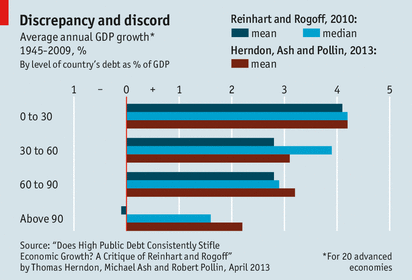
\includegraphics[width=.75\textwidth]{reinhart_rogoff.PNG}
\end{center}
\end{frame}


\begin{frame}{Motivation}
\begin{center}
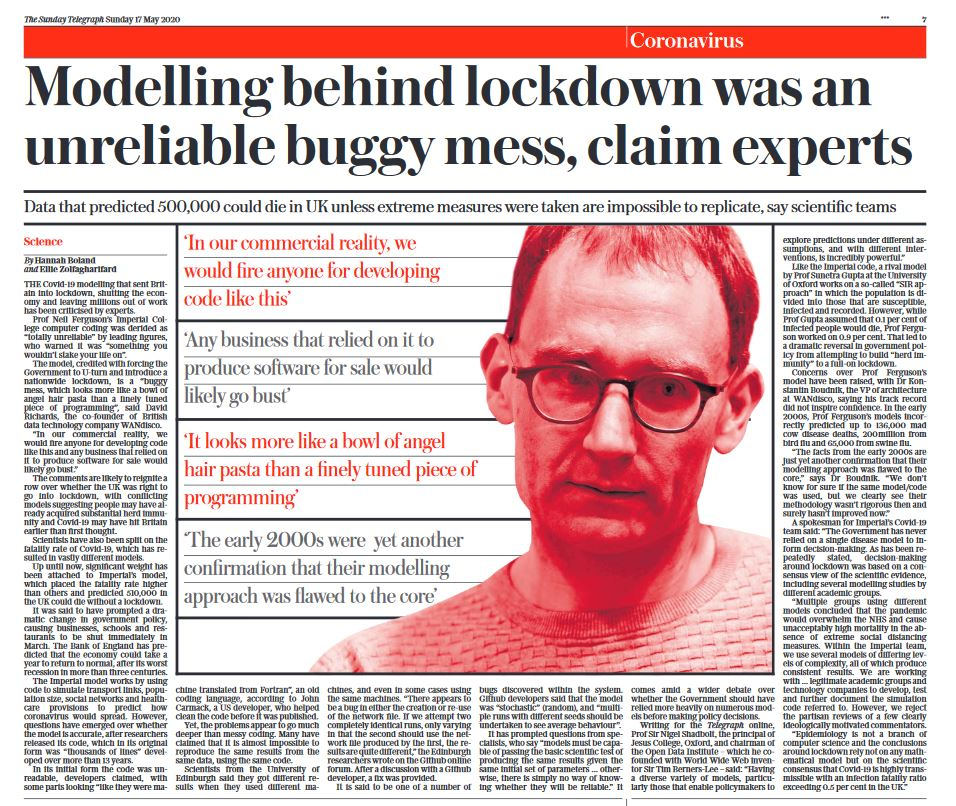
\includegraphics[width=.75\textwidth]{bad_code_media.JPG}
\end{center}
\end{frame}

\begin{frame}{Motivation}
Concept of Technical Debt
\begin{itemize}
  \item We write (messy) code for data cleaning/analyses
  \item We decide on data sets/models/graphs/tables/...
  \item We try to publish it, get a major revision
  \item We need to rerun some analyses
  \item Modifying/extending our code is more difficult than it should be
\end{itemize}
Solutions
\begin{itemize}
  \item Refactor/rewrite your could before submitting
  \item \textbf{Write better R code}
\end{itemize}
\end{frame}

\begin{frame}{Goals of this workshop}
\begin{itemize}
  \item Better practical R skills
  \item Better theoretical understanding of R (and programming)
  \item Different framing: R as a programming language
\end{itemize}
\end{frame}


\section{R Objects (Recap)}



\begin{frame}[fragile]
\begin{exampleblock}{}
  {\large ``To understand computations in R, two slogans are helpful: Everything that exists is an object. Everything that happens is a function call.''}
  \vskip5mm
  \hspace*\fill{\small--- John Chambers}
\end{exampleblock}
\end{frame}


\begin{frame}{R Objects (Recap)}

	\begin{itemize}
			\item What are objects?
			\item Attomic vectors
			\item Vector structures
			\item subsetting
			\item replacement
	\end{itemize}
\end{frame}


\subsection{What are objects?}


\begin{frame}{What are objects?}

	\begin{itemize}
			\item Data-structures that can be used in computations.
			\item Collections of data of al kinds that are dynamically created and manipulated.
			\item Can be very small, like a single number: \texttt{2.1}, or very big, like a complete data set  (i.e., \texttt{data.frame}) or a random forest output.
			\item Elementary data structures can be combined in more complex data structures.
			\item Creating new types of \emph{complex} objects is part of programming in R (S3, S4).
			
	\end{itemize}
\end{frame}


\subsection{Attomic Vectors}


\begin{frame}{Attomic Vectors}

\begin{center}
  \begin{tabular}{| l | l |}
    \hline
    \multicolumn{2}{|c|}{Basic object types} \\ \hline
    logical   & \texttt{TRUE}, \texttt{FALSE}, \texttt{NA} \\ 
    integer   & \texttt{1L}, \texttt{142}, \texttt{-5}, ..., \texttt{NA} \\
    double    & \texttt{1.0}, \texttt{1.25784}, \texttt{pi}, ..., \texttt{NA} \\
              & \texttt{NaN}, \texttt{-Inf}, \texttt{Inf} \\
    character & \texttt{"1"}, \texttt{"Some other string"}, ..., \texttt{NA} \\
    \hline
  \end{tabular}
\end{center}

mulitple values in one object $\rightarrow$ \texttt{length()} starting from \texttt{0}

\end{frame}


\begin{frame}[fragile]{Attomic Vectors}
An important type with special behavior is \texttt{NULL}. It is an empty object that can be interpreted as \emph{nothing}. It's length is 0.

\begin{knitrout}
\definecolor{shadecolor}{rgb}{0.933, 0.933, 0.933}\color{fgcolor}\begin{kframe}
\begin{alltt}
\hlkwd{c}\hlstd{(}\hlkwa{NULL}\hlstd{,} \hlstr{"a"}\hlstd{,} \hlkwa{NULL}\hlstd{)}
\hlkwd{length}\hlstd{(}\hlkwa{NULL}\hlstd{)}
\hlkwd{c}\hlstd{(}\hlkwa{NULL}\hlstd{,} \hlkwa{NULL}\hlstd{,} \hlkwa{NULL}\hlstd{)}
\end{alltt}
\end{kframe}
\end{knitrout}

\texttt{NULL} is mostly used as a default argument in fuction, in order to create some default behavior.

\end{frame}


\subsubsection{Coercion/Conversion}


\begin{frame}[fragile]{Coercion/Conversion}

	\begin{itemize}
			\item Automatic conversion:
			NULL $\rightarrow$ logical $\rightarrow$ integer $\rightarrow$ double $\rightarrow$ character
      \end{itemize}

\begin{knitrout}
\definecolor{shadecolor}{rgb}{0.933, 0.933, 0.933}\color{fgcolor}\begin{kframe}
\begin{alltt}
\hlnum{1} \hlopt{+} \hlnum{TRUE}
\hlkwd{c}\hlstd{(}\hlnum{FALSE}\hlstd{,} \hlstr{"word"}\hlstd{)}
\end{alltt}
\end{kframe}
\end{knitrout}

	\begin{itemize}		
			\item explicit conversion: \texttt{as."type"()}
	\end{itemize}
			
\begin{knitrout}
\definecolor{shadecolor}{rgb}{0.933, 0.933, 0.933}\color{fgcolor}\begin{kframe}
\begin{alltt}
\hlkwd{as.character}\hlstd{(}\hlnum{FALSE}\hlstd{)}
\hlkwd{as.logical}\hlstd{(}\hlnum{0}\hlopt{:}\hlnum{5}\hlstd{)}
\end{alltt}
\end{kframe}
\end{knitrout}

\end{frame}


\begin{frame}[fragile]{Attomic vectors - check type}

	\begin{itemize}	
			\item check type using: \texttt{is."type"()}
	\end{itemize}
  
\begin{knitrout}
\definecolor{shadecolor}{rgb}{0.933, 0.933, 0.933}\color{fgcolor}\begin{kframe}
\begin{alltt}
\hlkwd{is.logical}\hlstd{(}\hlnum{FALSE}\hlstd{)}
\hlkwd{is.character}\hlstd{(}\hlkwd{c}\hlstd{(}\hlnum{FALSE}\hlstd{,} \hlstr{"a string"}\hlstd{)[}\hlnum{1}\hlstd{])}
\end{alltt}
\end{kframe}
\end{knitrout}

	\begin{itemize}	
			\item check type using: \texttt{typeof()}
  \end{itemize}	
  
\begin{knitrout}
\definecolor{shadecolor}{rgb}{0.933, 0.933, 0.933}\color{fgcolor}\begin{kframe}
\begin{alltt}
\hlkwd{typeof}\hlstd{(}\hlnum{Inf}\hlstd{)}
\hlkwd{typeof}\hlstd{(}\hlnum{TRUE} \hlopt{+} \hlnum{FALSE}\hlstd{)}
\end{alltt}
\end{kframe}
\end{knitrout}

\end{frame}


\subsubsection{Assignment}


\begin{frame}[fragile]{Assignment}

In order to compute with objects efficiently, names can be assigned to the objects Using \texttt{<-} (or \texttt{=})

	
\begin{knitrout}
\definecolor{shadecolor}{rgb}{0.933, 0.933, 0.933}\color{fgcolor}\begin{kframe}
\begin{alltt}
\hlstd{my_object} \hlkwb{<-} \hlnum{TRUE}
\hlstd{my_object}
\end{alltt}
\end{kframe}
\end{knitrout}

The objects (with references) that are available to a user can be seen in the global environment using \texttt{ls}.

R overrides previous assignments without a message.


Removed objects (\texttt{rm(objectName)}) cannot be restored. $\rightarrow$ \emph{May the sourcecode be with you!}.

\end{frame}


\subsubsection{Attributes}


\begin{frame}[fragile]{Attributes}

Attributes can be attached to objects together with an name for that attribute. An attribute is itself an object. 

Attributes are easily lost in computations. (One of the reasons to use OOP with classes and methods.)

\begin{knitrout}
\definecolor{shadecolor}{rgb}{0.933, 0.933, 0.933}\color{fgcolor}\begin{kframe}
\begin{alltt}
\hlstd{my_object} \hlkwb{<-} \hlkwd{structure}\hlstd{(}\hlnum{5}\hlstd{,} \hlkwc{my_attribute} \hlstd{=} \hlstr{"string"}\hlstd{,} \hlkwc{other_attribute} \hlstd{=} \hlnum{FALSE}\hlstd{)}
\hlkwd{attributes}\hlstd{(my_object)}
\hlkwd{attr}\hlstd{(my_object,} \hlstr{"new"}\hlstd{)} \hlkwb{<-} \hlkwd{c}\hlstd{(}\hlnum{14}\hlstd{,} \hlnum{25}\hlstd{)}
\hlkwd{str}\hlstd{(my_object)}
\hlkwd{str}\hlstd{(}\hlkwd{as.integer}\hlstd{(my_object))}
\end{alltt}
\end{kframe}
\end{knitrout}

\end{frame}



\begin{frame}[fragile]{Attributes}

There are several attributes with a specific use: \texttt{"names"}, \texttt{"dim "}\texttt{"class"}, \texttt{"levels"}

\begin{itemize}
  \item \texttt{"names"} is a character vector that contains the names of elements of the vector/object. Names can be printed and set using \texttt{names(object) <- }.
  \item \texttt{"dim"} is an integer vector that specifies how we should interpret the vector (i.e., as a matrix, as an array). The dimensions of a vector can be printed and set using \texttt{dim(object) <- }.
  $\rightarrow$ a \texttt{matrix} or \texttt{matrix} is a vector with a \texttt{"dim"} attribute.
  \item \texttt{"class"} is a character vector that contains class names. Classes can be printed and set using \texttt{class(object) <- }}. See \textbf{Object Oriented Programming (S3)}
  \item \texttt{"levels"} is a character vector that contains the names levels of a factor. Levels can be printed and set using \texttt{levels(factor) <- }.
  \end{itemize}


\begin{knitrout}
\definecolor{shadecolor}{rgb}{0.933, 0.933, 0.933}\color{fgcolor}\begin{kframe}
\begin{alltt}
\hlstd{a} \hlkwb{<-} \hlnum{1}\hlopt{:}\hlnum{8}
\hlkwd{str}\hlstd{(a)}
\hlkwd{attr}\hlstd{(a,} \hlstr{"dim"}\hlstd{)} \hlkwb{<-} \hlkwd{c}\hlstd{(}\hlnum{2}\hlstd{,} \hlnum{4}\hlstd{)}
\hlkwd{str}\hlstd{(a)}
\hlkwd{is.matrix}\hlstd{(a)}
\hlkwd{as.character}\hlstd{(}\hlkwd{c}\hlstd{(}\hlkwc{aa} \hlstd{=} \hlnum{1}\hlstd{,} \hlkwc{bb} \hlstd{=} \hlnum{2}\hlstd{))}
\hlkwd{is.factor}\hlstd{(}\hlkwd{structure}\hlstd{(}\hlnum{1}\hlopt{:}\hlnum{2}\hlstd{,} \hlkwc{levels} \hlstd{=} \hlkwd{c}\hlstd{(}\hlstr{"a"}\hlstd{,} \hlstr{"b"}\hlstd{),} \hlkwc{class} \hlstd{=} \hlstr{"factor"}\hlstd{))}
\hlkwd{as.character}\hlstd{(}\hlkwd{c}\hlstd{(}\hlkwc{a} \hlstd{=} \hlnum{1}\hlstd{,} \hlkwc{b} \hlstd{=} \hlnum{2}\hlstd{))}
\end{alltt}
\end{kframe}
\end{knitrout}

\end{frame}


\begin{frame}[fragile]{Attributes}

A factor in R is actually an integer vector with a class attribute set to \texttt{"factor"}, and a levels attribute set to the level-labels that correspond to the integer values from 1 to the highest integer value in the integer vectors.

\begin{knitrout}
\definecolor{shadecolor}{rgb}{0.933, 0.933, 0.933}\color{fgcolor}\begin{kframe}
\begin{alltt}
\hlstd{int} \hlkwb{<-} \hlkwd{as.integer}\hlstd{(}\hlkwd{c}\hlstd{(}\hlnum{1}\hlstd{,} \hlnum{2}\hlstd{,} \hlnum{1}\hlstd{,} \hlnum{1}\hlstd{,} \hlnum{3}\hlstd{,} \hlnum{1}\hlstd{,} \hlnum{5}\hlstd{,} \hlnum{2}\hlstd{))}
\hlkwd{attr}\hlstd{(int,} \hlstr{"levels"}\hlstd{)} \hlkwb{<-} \hlkwd{c}\hlstd{(}\hlstr{"Now way!"}\hlstd{,} \hlstr{"Not sure"}\hlstd{,} \hlstr{"maybe"}\hlstd{,} \hlstr{"OK"}\hlstd{,} \hlstr{"Definitively!"}\hlstd{)}
\hlkwd{attr}\hlstd{(int,} \hlstr{"class"}\hlstd{)} \hlkwb{<-} \hlstr{"factor"}
\hlstd{int}
\end{alltt}
\end{kframe}
\end{knitrout}


\end{frame}



\begin{frame}{More Basic Object Types}

\begin{center}
  \begin{tabular}{| l | l |}
    \hline
    \multicolumn{2}{|c|}{More basic object types} \\ \hline
    complex     & \texttt{1 + 2.31i}, ... \texttt{NA} \\ 
    raw         & \texttt{as.raw(2)}, \texttt{charToRaw("a")} \\
    expression  & \texttt{expression(1+1, sum(a, b))} \\ \hline
    language    & a function call, \texttt{quote(1 + y)}  \\
    closure     & \texttt{function(x) x - 1}, \texttt{mean}  \\
    builtin     & \texttt{sum},  \texttt{c} \\
    special     & \texttt{for},  \texttt{return} \\ \hline
    environment & an environment \\
    symbol      & \texttt{quote(x)} \\ \hline
    ...         & ... \\
    \hline
  \end{tabular}
\end{center}

\end{frame}


\subsection{Vecture Structures}


\begin{frame}[fragile]{Vector Structures}

\begin{center}
  \begin{tabular}{| l | l |}
    \hline
    \multicolumn{2}{|c|}{More basic object types} \\ \hline
    matrix      & actually a vector with \texttt{"dim"} argument: two dimensions \\
                & \texttt{matrix()} \texttt{as.matrix()} \\ 
                & matrix algebra \\ 
    array       & actually a vector with with \texttt{"dim"} argument \\            \hline
    list        & \texttt{list()}, \texttt{as.list()}, ...  \\ 
    data.frame  & actually a list with vectors of equal length  \\
                & \texttt{data.frame}, \texttt{as.dataframe}  \\

    \hline
  \end{tabular}
\end{center}

\end{frame}



\begin{frame}[fragile]{List}

\begin{itemize}
  \item ``vectors'' that can contain any type of element
  \item including lists $\rightarrow$ recursive
  \item can have attributes, even \texttt{"dim"} (though mostly not useful)
\end{itemize}

\begin{knitrout}
\definecolor{shadecolor}{rgb}{0.933, 0.933, 0.933}\color{fgcolor}\begin{kframe}
\begin{alltt}
\hlstd{my_list} \hlkwb{<-} \hlkwd{list}\hlstd{(}\hlnum{1.23}\hlstd{,} \hlstr{"this"}\hlstd{,} \hlkwc{a} \hlstd{=} \hlkwd{list}\hlstd{(}\hlkwc{a} \hlstd{=} \hlkwd{c}\hlstd{(}\hlnum{1}\hlopt{:}\hlnum{2}\hlstd{)),} \hlnum{TRUE}\hlstd{)}
\hlkwd{attr}\hlstd{(my_list,} \hlstr{"dim"}\hlstd{)} \hlkwb{<-} \hlkwd{c}\hlstd{(}\hlnum{2}\hlstd{,} \hlnum{2}\hlstd{)}
\hlstd{my_list}  \hlcom{# printing fails}
\end{alltt}
\end{kframe}
\end{knitrout}

\end{frame}



\begin{frame}[fragile]{Data.frame}

\begin{itemize}
  \item a list of (named) vectors of equal length
  \item including lists (using \texttt{I()}).
  \item has row names (but ignore these)
  \item has dimensions (but not a \texttt{"dim"}-attribute)
\end{itemize}

\begin{knitrout}
\definecolor{shadecolor}{rgb}{0.933, 0.933, 0.933}\color{fgcolor}\begin{kframe}
\begin{alltt}
\hlstd{my_data}  \hlkwb{<-} \hlkwd{data.frame}\hlstd{(}\hlnum{1}\hlopt{:}\hlnum{4}\hlstd{,} \hlkwc{var1} \hlstd{=} \hlkwd{c}\hlstd{(}\hlstr{"a"}\hlstd{,} \hlstr{"b"}\hlstd{,} \hlstr{"c"}\hlstd{,} \hlstr{"d"}\hlstd{))}
\hlkwd{attributes}\hlstd{(my_data)}
\hlkwd{dim}\hlstd{(my_data)}
\hlkwd{names}\hlstd{(my_data)}
\hlkwd{typeof}\hlstd{(my_data)}
\hlkwd{data.frame}\hlstd{(}\hlnum{1}\hlopt{:}\hlnum{4}\hlstd{,} \hlkwc{var1} \hlstd{=} \hlkwd{I}\hlstd{(}\hlkwd{list}\hlstd{(}\hlkwd{c}\hlstd{(}\hlstr{"a"}\hlstd{,} \hlstr{"b"}\hlstd{),} \hlkwd{list}\hlstd{(}\hlnum{FALSE}\hlstd{,} \hlstr{"FALSE"}\hlstd{) ,} \hlnum{1}\hlopt{:}\hlnum{5}\hlstd{,} \hlkwd{c}\hlstd{(}\hlstr{"c"}\hlstd{,} \hlstr{"d"}\hlstd{))))}
\end{alltt}
\end{kframe}
\end{knitrout}

\end{frame}



\begin{frame}[fragile]{Matrix \& Array}

\begin{itemize}
  \item a vector with a \texttt{"dim"}-attribute
  \item mostly usefull for numeric vectors (integer and double)
  \item matrix algebra!  \texttt{t(matrix)}, \texttt{\%*\%}, \texttt{aperm(array))}...
  \item matrix has two dimensions, array has $n$ dimensions
\end{itemize}

\begin{knitrout}
\definecolor{shadecolor}{rgb}{0.933, 0.933, 0.933}\color{fgcolor}\begin{kframe}
\begin{alltt}
\hlstd{my_matrix} \hlkwb{<-} \hlkwd{matrix}\hlstd{(}\hlnum{2.5}\hlstd{,} \hlkwc{nrow} \hlstd{=} \hlnum{3}\hlstd{,} \hlkwc{ncol} \hlstd{=} \hlnum{3}\hlstd{)}
\hlkwd{is.array}\hlstd{(my_matrix)}
\hlkwd{dim}\hlstd{(my_matrix)}
\hlkwd{typeof}\hlstd{(my_matrix)}
\hlkwd{as.double}\hlstd{(my_matrix)}
\hlstd{my_array} \hlkwb{<-} \hlkwd{array}\hlstd{(}\hlnum{1}\hlopt{:}\hlnum{8}\hlstd{,} \hlkwc{dim} \hlstd{=} \hlkwd{c}\hlstd{(}\hlnum{2}\hlstd{,} \hlnum{2}\hlstd{,} \hlnum{2}\hlstd{))}
\hlkwd{is.array}\hlstd{(my_array)}
\hlkwd{dim}\hlstd{(my_array)}
\hlkwd{typeof}\hlstd{(my_array)}
\hlkwd{length}\hlstd{(my_array)}
\end{alltt}
\end{kframe}
\end{knitrout}

\end{frame}


\subsection{Subsetting - Selection}


\subsubsection{Subsetting - Attomic Vectors}


\begin{frame}[fragile]{Subsetting - attomic vectors}

A subset of elements from a vector can be accessed using \texttt{object[selection]}, where \texttt{selection} is:

\begin{itemize}
  \item a logical vector with the same length of the original vector (\texttt{TRUE}: select; \texttt{FALSE}: don't select)
  \item an integer vector indicating the indeces of the elements to select (or exclude)
  \item a character vector with the names of the elements to select
\end{itemize}

\end{frame}


\begin{frame}{Subsetting - attomic vectors}

Using a logical vector:

\begin{itemize}
  \item the logical vector should have the same length of the object. If shorter, the logical is repeated; if longer, \texttt{NA}s are added if \texttt{TRUE}. $\rightarrow$ always use the same length!
  \item handy when you want to select based on a condition related to the object values
\end{itemize}

\end{frame}


\begin{frame}[fragile]{Subsetting - attomic vectors}
\begin{knitrout}
\definecolor{shadecolor}{rgb}{0.933, 0.933, 0.933}\color{fgcolor}\begin{kframe}
\begin{alltt}
\hlstd{my_object} \hlkwb{<-} \hlkwd{c}\hlstd{(}\hlkwc{a} \hlstd{=} \hlnum{1}\hlstd{,} \hlkwc{b} \hlstd{=} \hlnum{5}\hlstd{,} \hlkwc{c} \hlstd{=} \hlnum{3}\hlstd{,} \hlkwc{d} \hlstd{=} \hlnum{8}\hlstd{)}
\hlstd{my_object[}\hlkwd{c}\hlstd{(}\hlnum{TRUE}\hlstd{,} \hlnum{FALSE}\hlstd{,} \hlnum{FALSE}\hlstd{,} \hlnum{TRUE}\hlstd{)]}
\hlstd{my_object[}\hlnum{TRUE}\hlstd{]}
\hlstd{my_object[}\hlkwd{c}\hlstd{(}\hlnum{FALSE}\hlstd{,} \hlnum{TRUE}\hlstd{)]}
\hlstd{my_object[}\hlkwd{c}\hlstd{(}\hlnum{FALSE}\hlstd{,} \hlnum{TRUE}\hlstd{,} \hlnum{TRUE}\hlstd{,} \hlnum{FALSE}\hlstd{,} \hlnum{TRUE}\hlstd{)]}
\hlstd{my_object[my_object} \hlopt{>} \hlnum{4}\hlstd{]}
\hlstd{my_object[}\hlnum{1}\hlopt{:}\hlnum{4} \hlopt{<} \hlnum{4}\hlstd{]}
\end{alltt}
\end{kframe}
\end{knitrout}

\end{frame}


\begin{frame}{Subsetting - attomic vectors}

Using an integer vector:

\begin{itemize}
  \item the integer vector can have any length (repeated indices are repeatedly selected)
  \item positive values mean \emph{select}, negative values mean \emph{drop}
  \item positive and negative values cannot be combined
  \item for integers higher than the number of elements in the vector, \texttt{NA}s are added
  \item using \texttt{which()} a logical vector is transformed in an integer vector with the indices of the elements that were \texttt{TRUE}
  \item double elements are truncated towards zero (using \texttt{as.integer()}))
\end{itemize}

\end{frame}

\begin{frame}[fragile]{Subsetting - attomic vectors}
\begin{knitrout}
\definecolor{shadecolor}{rgb}{0.933, 0.933, 0.933}\color{fgcolor}\begin{kframe}
\begin{alltt}
\hlstd{my_object} \hlkwb{<-} \hlkwd{c}\hlstd{(}\hlkwc{a} \hlstd{=} \hlnum{1}\hlstd{,} \hlkwc{b} \hlstd{=} \hlnum{5}\hlstd{,} \hlkwc{c} \hlstd{=} \hlnum{3}\hlstd{,} \hlkwc{d} \hlstd{=} \hlnum{8}\hlstd{)}
\hlstd{my_object[}\hlkwd{c}\hlstd{(}\hlnum{1}\hlstd{,} \hlnum{5}\hlstd{)]}
\hlstd{my_object[}\hlkwd{c}\hlstd{(}\hlnum{1}\hlstd{,} \hlnum{2}\hlstd{,} \hlnum{1}\hlstd{,} \hlnum{2}\hlstd{,} \hlnum{1}\hlstd{,} \hlnum{2}\hlstd{,} \hlnum{1} \hlstd{,}\hlnum{2}\hlstd{,} \hlnum{1}\hlstd{,} \hlnum{2}\hlstd{,} \hlnum{1}\hlstd{,} \hlnum{2}\hlstd{)]}
\hlstd{my_object[}\hlopt{-}\hlkwd{c}\hlstd{(}\hlnum{2}\hlstd{,} \hlnum{4}\hlstd{,} \hlnum{2}\hlstd{)]}
\hlstd{my_object[my_object} \hlopt{>} \hlnum{4}\hlstd{]}
\hlstd{my_object[}\hlkwd{which}\hlstd{(my_object} \hlopt{>} \hlnum{4}\hlstd{)]}
\hlkwd{which}\hlstd{(my_object} \hlopt{>} \hlnum{4}\hlstd{)}
\hlstd{my_object[}\hlnum{1.999}\hlstd{]}
\end{alltt}
\end{kframe}
\end{knitrout}

\end{frame}



\begin{frame}{Subsetting - attomic vectors}

Using a character vector:

\begin{itemize}
  \item the strings that match with the names of the elements in the vector are returned
  \item the character vector can have any length (repeated names are repeatedly selected)
  \item only selection is possible (dropping is not)
  \item strings that are not matched with names return \texttt{NA}
\end{itemize}

\end{frame}

\begin{frame}[fragile]{Subsetting - attomic vectors}
\begin{knitrout}
\definecolor{shadecolor}{rgb}{0.933, 0.933, 0.933}\color{fgcolor}\begin{kframe}
\begin{alltt}
\hlstd{my_object} \hlkwb{<-} \hlkwd{c}\hlstd{(}\hlkwc{a} \hlstd{=} \hlnum{1}\hlstd{,} \hlkwc{b} \hlstd{=} \hlnum{5}\hlstd{,} \hlkwc{c} \hlstd{=} \hlnum{3}\hlstd{,} \hlkwc{d} \hlstd{=} \hlnum{8}\hlstd{)}
\hlstd{my_object[}\hlkwd{c}\hlstd{(}\hlstr{"a"}\hlstd{,} \hlstr{"b"}\hlstd{)]}
\hlstd{my_object[}\hlkwd{c}\hlstd{(}\hlstr{"a"}\hlstd{,} \hlstr{"b"}\hlstd{,} \hlstr{"a"}\hlstd{,} \hlstr{"b"}\hlstd{,} \hlstr{"a"}\hlstd{,} \hlstr{"b"}\hlstd{,} \hlstr{"a"}\hlstd{,} \hlstr{"b"}\hlstd{,} \hlstr{"a"}\hlstd{,} \hlstr{"b"}\hlstd{,} \hlstr{"a"}\hlstd{,} \hlstr{"b"}\hlstd{)]}
\hlstd{my_object[}\hlopt{-}\hlkwd{c}\hlstd{(}\hlstr{"a"}\hlstd{,} \hlstr{"b"}\hlstd{)]}
\end{alltt}


{\ttfamily\noindent\bfseries\color{errorcolor}{\#\# Error in -c("{}a"{}, "{}b"{}): invalid argument to unary operator}}\end{kframe}
\end{knitrout}

\end{frame}



\begin{frame}[fragile]{Subsetting - attomic vectors}

A \textbf{sinlge} element from a vector can be accessed using \texttt{object[[selection]}, where \texttt{selection} is:

\begin{itemize}
  \item an integer value indicating the index of the element to select
  \item a character vector with the names of the elements to select
\end{itemize}

\begin{knitrout}
\definecolor{shadecolor}{rgb}{0.933, 0.933, 0.933}\color{fgcolor}\begin{kframe}
\begin{alltt}
\hlstd{my_object} \hlkwb{<-} \hlkwd{c}\hlstd{(}\hlkwc{a} \hlstd{=} \hlnum{1}\hlstd{,} \hlkwc{b} \hlstd{=} \hlnum{5}\hlstd{,} \hlkwc{c} \hlstd{=} \hlnum{3}\hlstd{,} \hlkwc{c2} \hlstd{=} \hlnum{8}\hlstd{)}
\hlstd{my_object[[}\hlnum{2}\hlstd{]]}
\hlstd{my_object[[}\hlstr{"c"}\hlstd{]]}
\end{alltt}
\end{kframe}
\end{knitrout}

\end{frame}


\subsubsection{Subsetting - Matrix \& Arrays}


\begin{frame}[fragile]{Subsetting - Matrix \& Arrays}

Because arrays and martrices are attomic vectors (with a \texttt{"dim"} argument), the rules for attomic vectors apply.

In addition, selection is possible per dimension:

\begin{itemize}
  \item multiple selection vectors separated by a comma
  \item selection vectors can be character (match row or column names), integer (row and column number) or logical
  \item the first vector selects the rows, the second the columns (and so on)
  \item automatically the dimensions are dropped. Use \texttt{drop = FALSE} to avoid this
\end{itemize}

Finally, the selection ellement can also be a matrix (with one column per dimension). Each row in the matrix selects one value.

\begin{knitrout}
\definecolor{shadecolor}{rgb}{0.933, 0.933, 0.933}\color{fgcolor}\begin{kframe}
\begin{alltt}
\hlstd{my_matrix} \hlkwb{<-} \hlkwd{matrix}\hlstd{(}\hlkwd{c}\hlstd{(}\hlnum{11}\hlstd{,} \hlnum{12}\hlstd{,} \hlnum{21}\hlstd{,} \hlnum{22}\hlstd{),} \hlkwc{ncol} \hlstd{=} \hlnum{2}\hlstd{,} \hlkwc{dimnames} \hlstd{=} \hlkwd{list}\hlstd{(}\hlkwd{paste0}\hlstd{(}\hlstr{"row"}\hlstd{,} \hlnum{1}\hlopt{:}\hlnum{2}\hlstd{),} \hlkwd{paste0}\hlstd{(}\hlstr{"col"}\hlstd{,} \hlnum{1}\hlopt{:}\hlnum{2}\hlstd{)))}
\hlkwd{names}\hlstd{(my_matrix)} \hlkwb{<-} \hlstd{letters[}\hlnum{1}\hlopt{:}\hlnum{4}\hlstd{]}
\hlstd{my_matrix[}\hlnum{2}\hlstd{]}
\hlstd{my_matrix[[}\hlstr{"b"}\hlstd{]]}
\hlstd{my_matrix[my_matrix} \hlopt{<} \hlnum{20}\hlstd{]}
\hlstd{my_matrix[}\hlnum{2}\hlstd{,]}
\hlstd{my_matrix[,}\hlnum{2}\hlstd{]}
\hlstd{my_matrix[}\hlopt{-}\hlnum{1}\hlstd{,}\hlstr{"col2"}\hlstd{]}
\hlstd{my_matrix[}\hlstr{"row1"}\hlstd{,}\hlkwd{c}\hlstd{(}\hlnum{TRUE}\hlstd{,} \hlnum{FALSE}\hlstd{)]}
\hlstd{my_matrix[}\hlstr{"row1"}\hlstd{,}\hlkwd{c}\hlstd{(}\hlnum{TRUE}\hlstd{,} \hlnum{FALSE}\hlstd{)]}
\hlkwd{is.matrix}\hlstd{(my_matrix[,}\hlnum{1}\hlstd{])}
\hlkwd{is.matrix}\hlstd{(my_matrix[,}\hlnum{1}\hlstd{,} \hlkwc{drop} \hlstd{=} \hlnum{FALSE}\hlstd{])}
\hlstd{my_matrix[}\hlkwd{matrix}\hlstd{(}\hlkwd{c}\hlstd{(}\hlkwd{c}\hlstd{(}\hlnum{1}\hlstd{,} \hlnum{2}\hlstd{),} \hlkwd{c}\hlstd{(}\hlnum{1}\hlstd{,} \hlnum{2}\hlstd{)),} \hlkwc{ncol} \hlstd{=} \hlnum{2}\hlstd{)]}
\end{alltt}
\end{kframe}
\end{knitrout}

\end{frame}


\subsubsection{Subsetting - Vector Structures}


\begin{frame}[fragile]{Subsetting - Lists}

\begin{itemize}
  \item For list, the rules are similar as for atomic vectors.
  \item \texttt{list[selection]} gives a list
  \item \texttt{list[[selection]]} gives the element (which can be a list)
  \item \texttt{list[["element\_name"]]} is the same as \texttt{list\$element\_name}
\end{itemize}

\begin{knitrout}
\definecolor{shadecolor}{rgb}{0.933, 0.933, 0.933}\color{fgcolor}\begin{kframe}
\begin{alltt}
\hlstd{my_list}\hlkwb{<-} \hlkwd{list}\hlstd{(}\hlkwc{a} \hlstd{=} \hlnum{1}\hlstd{,} \hlkwc{b} \hlstd{=} \hlnum{5}\hlstd{,} \hlkwc{c} \hlstd{=} \hlnum{3}\hlstd{,} \hlkwc{d} \hlstd{=} \hlnum{8}\hlstd{)}
\hlstd{my_list[}\hlkwd{c}\hlstd{(}\hlnum{2}\hlstd{,} \hlnum{2}\hlstd{)]}
\hlstd{my_list[[}\hlstr{"b"}\hlstd{]]}
\hlstd{my_list}\hlopt{$}\hlstd{b}
\hlstd{my_list[}\hlkwd{c}\hlstd{(}\hlnum{TRUE}\hlstd{,} \hlnum{TRUE}\hlstd{,} \hlnum{FALSE}\hlstd{)]}
\hlkwd{is.list}\hlstd{(my_list[}\hlstr{"a"}\hlstd{])}
\hlkwd{is.list}\hlstd{(my_list[[}\hlstr{"a"}\hlstd{]])}
\end{alltt}
\end{kframe}
\end{knitrout}

\end{frame}


\begin{frame}[fragile]{Subsetting - data.frames}

Because data.frames are lists, the rules for lists apply. 

In addition, the selection rules for matrices can be used: (i.e., with ).

\begin{itemize}
  \item selection per row and column
  \item selection via a matrix with two columns
\end{itemize}

\begin{knitrout}
\definecolor{shadecolor}{rgb}{0.933, 0.933, 0.933}\color{fgcolor}\begin{kframe}
\begin{alltt}
\hlstd{my_dat} \hlkwb{<-} \hlkwd{data.frame}\hlstd{(}\hlkwc{col1} \hlstd{=} \hlkwd{c}\hlstd{(}\hlnum{11}\hlstd{,} \hlnum{21}\hlstd{),} \hlkwc{col2} \hlstd{=} \hlkwd{c}\hlstd{(}\hlnum{12}\hlstd{,} \hlnum{22}\hlstd{))}
\hlstd{my_dat[}\hlnum{1}\hlstd{]}
\hlstd{my_dat[}\hlstr{"col1"}\hlstd{]}
\hlstd{my_dat[,}\hlstr{"col1"}\hlstd{]}
\hlstd{my_dat[,}\hlstr{"col1"}\hlstd{,} \hlkwc{drop} \hlstd{=} \hlnum{FALSE}\hlstd{]}
\hlstd{my_dat}\hlopt{$}\hlstd{col1}
\hlstd{my_dat[}\hlkwd{c}\hlstd{(}\hlnum{TRUE}\hlstd{,} \hlnum{FALSE}\hlstd{)]}
\hlkwd{is.data.frame}\hlstd{(my_dat[}\hlstr{"col1"}\hlstd{])}
\hlkwd{is.data.frame}\hlstd{(my_dat[[}\hlstr{"col1"}\hlstd{]])}
\hlstd{my_dat[}\hlkwd{c}\hlstd{(}\hlnum{TRUE}\hlstd{,} \hlnum{FALSE}\hlstd{),} \hlstr{"col2"}\hlstd{]}
\hlstd{my_dat[}\hlkwd{c}\hlstd{(}\hlnum{TRUE}\hlstd{,} \hlnum{FALSE}\hlstd{),} \hlstr{"col2"}\hlstd{,} \hlkwc{drop} \hlstd{=} \hlnum{FALSE}\hlstd{]}
\hlstd{my_dat[}\hlkwd{matrix}\hlstd{(}\hlkwd{c}\hlstd{(}\hlkwd{c}\hlstd{(}\hlnum{1}\hlstd{,} \hlnum{2}\hlstd{),} \hlkwd{c}\hlstd{(}\hlnum{1}\hlstd{,} \hlnum{2}\hlstd{)),} \hlkwc{ncol} \hlstd{=} \hlnum{2}\hlstd{)]}
\end{alltt}
\end{kframe}
\end{knitrout}

\end{frame}


\subsection{Element Replacement}


\begin{frame}[fragile]{Element Replacement}

A subset of elements from a vector or vector structure can be replaced using \texttt{object[selection] <- new\_values}:

\begin{itemize}
  \item the modifications are done in place
  \item the structure and class of the object stay unchanged
  \item the length of the new values should correspond with the length of the selection (the number of elements to replace should be a multiple of the number of new values)
  \item only for lists, the replacement can be \texttt{NULL} (which removes the element from the list)
\end{itemize}

\begin{knitrout}
\definecolor{shadecolor}{rgb}{0.933, 0.933, 0.933}\color{fgcolor}\begin{kframe}
\begin{alltt}
\hlstd{my_dat} \hlkwb{<-} \hlkwd{data.frame}\hlstd{(}\hlkwc{col1} \hlstd{=} \hlkwd{c}\hlstd{(}\hlnum{11}\hlstd{,} \hlnum{21}\hlstd{),} \hlkwc{col2} \hlstd{=} \hlkwd{c}\hlstd{(}\hlnum{12}\hlstd{,} \hlnum{22}\hlstd{))}
\hlstd{my_dat[}\hlnum{1}\hlstd{]} \hlkwb{<-} \hlnum{33}
\hlstd{my_dat[}\hlstr{"col2"}\hlstd{]} \hlkwb{<-} \hlkwa{NULL}
\hlstd{my_dat[,}\hlnum{1}\hlstd{]} \hlkwb{<-} \hlkwa{NULL}
\end{alltt}
\end{kframe}
\end{knitrout}
\end{frame}


\begin{frame}[fragile]
\begin{exampleblock}{}
  {\large ``To understand computations in R, two slogans are helpful: Everything that exists is an object. Everything that happens is a function call.''}
  \vskip5mm
  \hspace*\fill{\small--- John Chambers}
\end{exampleblock}
\end{frame}


\subsection{Function Calls}


\begin{frame}{Function Calls}

\begin{itemize}
  \item Computing in R happens through function calls. A function is applied to one or more objects, and returns an object after the computation. 
  \item The typical use is \texttt{function\_name(object1, argument\_name = object2)}
  \item Computations that seem not to be done using functions are actually also functions. Check \texttt{\`<-\`(a, 5)} or \texttt{\`>\`(5, 2)}
  \item most functions that seem not to return an object, return it invisibly. Check \texttt{(`<-`(a, 5))}.
\end{itemize}

\end{frame}


\section{Clean Code}


\begin{frame}{Clean Code}

\begin{itemize}
  \item Code Style 
  \item Efficient R
  \item Efficient RStudio
\end{itemize}

\end{frame}


\subsection{Code Style}


\begin{frame}[fragile]
\begin{exampleblock}{}
  {\large ``Write code for humans, not for machines!''}
  \vskip5mm
  \hspace*\fill{\small}
\end{exampleblock}
\end{frame}



\begin{frame}{Code Style}

Invest time in writing readable R-code.

\begin{itemize}
  \item It will make collaboration easier
  \item It will make debugging easier
  \item It will help make your analysis reproducible 
\end{itemize}

There is a complete \emph{tidyverse} style-guide \url{https://style.tidyverse.org/}.

\end{frame}


\subsection{Go easy on your eyes}

\begin{frame}{Go easy on your eyes}

\begin{itemize}
  \item with spaces before and after: \texttt{-  +  /  *  =  <-  <  ==  > }
  \item always use \texttt{<-} for assignments
  \item only use \texttt{=} in function calls
  \item use indentation (largely automatical in RStudio)
  \item \texttt{CamelCaseNames} vs \texttt{snake\_case\_names}
  \item be consistent!
  \item wrap long lines at column 70-80 (Rstudio)
\end{itemize}

\end{frame}


\begin{frame}[fragile]{White spaces}

\begin{knitrout}
\definecolor{shadecolor}{rgb}{0.933, 0.933, 0.933}\color{fgcolor}\begin{kframe}
\begin{alltt}
\hlstd{new_var}\hlkwb{=}\hlstd{(var1}\hlopt{*}\hlstd{var2}\hlopt{/}\hlnum{2}\hlstd{)}\hlopt{-}\hlnum{5}\hlopt{/}\hlstd{(var3}\hlopt{+}\hlstd{var4)}

\hlcom{# versus}

\hlstd{new_var} \hlkwb{<-} \hlstd{(var1} \hlopt{*} \hlstd{var2} \hlopt{/} \hlnum{2}\hlstd{)} \hlopt{-} \hlnum{5} \hlopt{/} \hlstd{(var3} \hlopt{+} \hlstd{var4)}
\end{alltt}
\end{kframe}
\end{knitrout}

\end{frame}


\begin{frame}[fragile]{Indentation}

\begin{knitrout}
\definecolor{shadecolor}{rgb}{0.933, 0.933, 0.933}\color{fgcolor}\begin{kframe}
\begin{alltt}
\hlkwa{for}\hlstd{(name} \hlkwa{in} \hlstd{names)\{formula}\hlkwb{=}\hlkwd{as.formula}\hlstd{(}\hlkwd{paste0}\hlstd{(}\hlstr{"y~.-"}\hlstd{,name))}
\hlstd{fit}\hlkwb{<-}\hlkwd{lm}\hlstd{(formula,}\hlkwc{data}\hlstd{=my_data)}
\hlstd{coefs[[}\hlstr{"name"}\hlstd{]]}\hlkwb{=}\hlkwd{coef}\hlstd{(fit)}
\hlkwd{print}\hlstd{(name)}
\hlkwd{print}\hlstd{(}\hlkwd{summary}\hlstd{(fit))\}}

\hlcom{# versus}

\hlkwa{for}\hlstd{(name} \hlkwa{in} \hlstd{names)\{}
  \hlstd{formula} \hlkwb{<-} \hlkwd{as.formula}\hlstd{(}\hlkwd{paste0}\hlstd{(}\hlstr{"y~.-"}\hlstd{, name))}
  \hlstd{fit} \hlkwb{<-} \hlkwd{lm}\hlstd{(formula,} \hlkwc{data} \hlstd{= my_data)}
  \hlstd{coefs[[}\hlstr{"name"}\hlstd{]]} \hlkwb{<-} \hlkwd{coef}\hlstd{(fit)}
  \hlkwd{print}\hlstd{(name)}
  \hlkwd{print}\hlstd{(}\hlkwd{summary}\hlstd{(fit))}
\hlstd{\}}
\end{alltt}
\end{kframe}
\end{knitrout}

\end{frame}


\begin{frame}[fragile]{Wrap long lines}

\begin{knitrout}
\definecolor{shadecolor}{rgb}{0.933, 0.933, 0.933}\color{fgcolor}\begin{kframe}
\begin{alltt}
\hlstd{final_results} \hlkwb{<-} \hlkwd{data.frame}\hlstd{(}\hlkwc{first_variable} \hlstd{=} \hlkwd{sqrt}\hlstd{(results}\hlopt{$}\hlstd{mean_squared_error),} \hlkwc{second_variable} \hlstd{=} \hlkwd{paste0}\hlstd{(results}\hlopt{$}\hlstd{condition, results}\hlopt{$}\hlstd{class,} \hlkwc{sep} \hlstd{=} \hlstr{":"}\hlstd{),} \hlkwc{third_variable} \hlstd{= results}\hlopt{$}\hlstd{bias)}

\hlcom{# versus}

\hlstd{final_results} \hlkwb{<-} \hlkwd{data.frame}\hlstd{(}
  \hlkwc{first_variable} \hlstd{=} \hlkwd{sqrt}\hlstd{(results}\hlopt{$}\hlstd{mean_squared_error),}
  \hlkwc{second_variable} \hlstd{=} \hlkwd{paste0}\hlstd{(results}\hlopt{$}\hlstd{condition, results}\hlopt{$}\hlstd{class,} \hlkwc{sep} \hlstd{=} \hlstr{":"}\hlstd{),}
  \hlkwc{third_variable} \hlstd{= results}\hlopt{$}\hlstd{bias)}
\end{alltt}
\end{kframe}
\end{knitrout}

\end{frame}



\subsection{Go easy on your mind}

\begin{frame}{Go easy on your mind}

\begin{itemize}
  \item use meaningful names: ``self-explainable''
  \item benefit from autocompletion (\texttt{tab}) => embrace longer names
  \item always write the formal arguments in function calls (except the first)
  \item use \texttt{TRUE} and \texttt{FALSE} not \texttt{T} and \texttt{F}
  \item comment, comment, comment
  \begin{itemize}
    \item NOT what (should be clear from the code)
    \item BUT why
    \item Explain the reasoning, not the code 
  \end{itemize}
\end{itemize}

\end{frame}


\begin{frame}[fragile]{Write formal arguments}

Benefit from auto completion using \texttt{tab}

\begin{knitrout}
\definecolor{shadecolor}{rgb}{0.933, 0.933, 0.933}\color{fgcolor}\begin{kframe}
\begin{alltt}
\hlstd{m1_B} \hlkwb{<-} \hlkwd{lm}\hlstd{(outcome} \hlopt{~} \hlstd{age}\hlopt{*}\hlstd{gender, exp1, condition_1, freq)}

\hlcom{# versus}

\hlstd{lm_age_gender} \hlkwb{<-} \hlkwd{lm}\hlstd{(outcome} \hlopt{~} \hlstd{age}\hlopt{*}\hlstd{gender,} \hlkwc{data} \hlstd{= exp1,}
                    \hlkwc{subset} \hlstd{= condition_1,}
                    \hlkwc{weigths} \hlstd{= freq)}
\end{alltt}
\end{kframe}
\end{knitrout}

\end{frame}



\begin{frame}[fragile]{Use meaningful names}

\begin{knitrout}
\definecolor{shadecolor}{rgb}{0.933, 0.933, 0.933}\color{fgcolor}\begin{kframe}
\begin{alltt}
\hlstd{V} \hlkwb{<-} \hlkwd{myFun}\hlstd{(m1_B)}

\hlcom{# versus}

\hlstd{RMSE_age_gender} \hlkwb{<-} \hlkwd{get_RMSE}\hlstd{(lm_age_gender)}
\end{alltt}
\end{kframe}
\end{knitrout}

Use \texttt{verbs} for functions and \texttt{nouns} for objects.

\end{frame}


\begin{frame}[fragile]{Comment, comment, comment}

\begin{knitrout}
\definecolor{shadecolor}{rgb}{0.933, 0.933, 0.933}\color{fgcolor}\begin{kframe}
\begin{alltt}
\hlcom{## Start every Rscript with a comment that explains what the code in the script}
\hlcom{##  does, why it does this, and to which project it belongs. }
\hlcom{##  Your future self will be very thankful!}
\hlcom{##}
\hlcom{## Mention which packages you are using in this Rscript.}


\hlcom{## Use sections to separate chunks -------------------------------------------}


\hlcom{## Maybe even subsections ====================================================}


\hlcom{## Recode variables so that missings are coded as "NA"}
\hlstd{data[data} \hlopt \hlkwd{c}\hlstd{(}\hlnum{99}\hlstd{,} \hlnum{999}\hlstd{)]} \hlkwb{<-} \hlnum{NA}         \hlcom{# missings were coded as 99 or 999}
\end{alltt}
\end{kframe}
\end{knitrout}

\end{frame}


\subsection{R Peculiarities}

\begin{frame}[fragile]{Don't grow, replace}

\begin{knitrout}
\definecolor{shadecolor}{rgb}{0.933, 0.933, 0.933}\color{fgcolor}\begin{kframe}
\begin{alltt}
\hlstd{n} \hlkwb{<-} \hlnum{2e+4}
\hlstd{data} \hlkwb{<-} \hlkwd{data.frame}\hlstd{(}\hlkwc{x} \hlstd{=} \hlkwd{runif}\hlstd{(n),}
                   \hlkwc{y} \hlstd{=} \hlkwd{runif}\hlstd{(n),}
                   \hlkwc{z} \hlstd{=} \hlkwd{seq_len}\hlstd{(n))}

\hlcom{# grow object}
\hlkwd{system.time}\hlstd{(\{}
  \hlstd{new_data} \hlkwb{<-} \hlkwa{NULL}

  \hlkwa{for}\hlstd{(row_nr} \hlkwa{in} \hlkwd{seq_len}\hlstd{(}\hlkwd{NROW}\hlstd{(data)))\{}
    \hlstd{new_data} \hlkwb{<-} \hlkwd{cbind}\hlstd{(data[row_nr,],} \hlkwc{result} \hlstd{=} \hlkwd{exp}\hlstd{(data}\hlopt{$}\hlstd{x[row_nr])} \hlopt{/}
                        \hlkwd{log}\hlstd{(data}\hlopt{$}\hlstd{z[row_nr])} \hlopt{+} \hlnum{5} \hlopt{*} \hlkwd{sqrt}\hlstd{(data}\hlopt{$}\hlstd{y[row_nr]))}
  \hlstd{\}}
\hlstd{\})}

\hlcom{# replace}
\hlkwd{system.time}\hlstd{(\{}
  \hlstd{n_rows} \hlkwb{<-} \hlkwd{dim}\hlstd{(data)[}\hlnum{1}\hlstd{]}
  \hlstd{data}\hlopt{$}\hlstd{result} \hlkwb{<-} \hlkwd{rep}\hlstd{(}\hlnum{NA}\hlstd{, n_rows)}

  \hlkwa{for}\hlstd{(row_nr} \hlkwa{in} \hlkwd{seq_len}\hlstd{(n_rows))\{}
    \hlstd{data}\hlopt{$}\hlstd{result[row_nr]} \hlkwb{<-} \hlkwd{exp}\hlstd{(data}\hlopt{$}\hlstd{x[row_nr])} \hlopt{/} \hlkwd{log}\hlstd{(data}\hlopt{$}\hlstd{z[row_nr])} \hlopt{+}
      \hlnum{5} \hlopt{*} \hlkwd{sqrt}\hlstd{(data}\hlopt{$}\hlstd{y[row_nr])}
  \hlstd{\}}
\hlstd{\})}
\end{alltt}
\end{kframe}
\end{knitrout}

Replace preferably by column, not by row (in data.frames)

\end{frame}



\begin{frame}[fragile]{Vectorize}

\begin{knitrout}
\definecolor{shadecolor}{rgb}{0.933, 0.933, 0.933}\color{fgcolor}\begin{kframe}
\begin{alltt}
\hlstd{n} \hlkwb{<-} \hlnum{2e+4}
\hlstd{data} \hlkwb{<-} \hlkwd{data.frame}\hlstd{(}\hlkwc{x} \hlstd{=} \hlkwd{runif}\hlstd{(n),}
                   \hlkwc{y} \hlstd{=} \hlkwd{runif}\hlstd{(n),}
                   \hlkwc{z} \hlstd{=} \hlkwd{seq_len}\hlstd{(n))}

\hlcom{# vectorized}
\hlkwd{system.time}\hlstd{(\{}
  \hlstd{result} \hlkwb{<-} \hlkwd{exp}\hlstd{(data}\hlopt{$}\hlstd{x)} \hlopt{/} \hlkwd{log}\hlstd{(data}\hlopt{$}\hlstd{z)} \hlopt{+} \hlnum{5} \hlopt{*} \hlkwd{sqrt}\hlstd{(data}\hlopt{$}\hlstd{y)}
\hlstd{\})}
\end{alltt}
\end{kframe}
\end{knitrout}

\end{frame}



\begin{frame}[fragile]{Keep your code slim}

Try to limit your \emph{package-dependencies}. Only load (i.e., \texttt{library()}) the packages that you absolutely need. I you are only using \texttt{dplyr}, it does not make sense to load the complete \texttt{tidyverse}.

\textbf{Controversial:} when you are only using a function from a package once or twice, DON'T load the package, but directly access the function using the \texttt{::} operator.

Less loaded packages mean less changes or name conflicts.

\end{frame}


\begin{frame}[fragile]{Never Attach}

Forget about \texttt{attacht()}! Don't use it, unless you completely understand what happens (\texttt{?attach}).

With `data.frames`, use `with(data.frame, expression)` instead.

\begin{knitrout}
\definecolor{shadecolor}{rgb}{0.933, 0.933, 0.933}\color{fgcolor}\begin{kframe}
\begin{alltt}
\hlcom{# using with()}
\hlstd{n} \hlkwb{<-} \hlnum{2e+4}
\hlstd{data} \hlkwb{<-} \hlkwd{data.frame}\hlstd{(}\hlkwc{x} \hlstd{=} \hlkwd{runif}\hlstd{(n),}
                   \hlkwc{y} \hlstd{=} \hlkwd{runif}\hlstd{(n),}
                   \hlkwc{z} \hlstd{=} \hlkwd{seq_len}\hlstd{(n))}
\hlstd{result} \hlkwb{<-} \hlkwd{with}\hlstd{(data,} \hlkwd{exp}\hlstd{(x)} \hlopt{/} \hlkwd{log}\hlstd{(z)} \hlopt{+} \hlnum{5} \hlopt{*} \hlkwd{sqrt}\hlstd{(y))}
\end{alltt}
\end{kframe}
\end{knitrout}

\end{frame}



\begin{frame}[fragile]{Testing R code}

Writing code is error prone. Incorporate tests and checks in your workflow. For instance, when you do data manipulations like a complex restructuring of the data, or a complex recoding of multiple variable, write some code that allows you the check whether the obtained results are what you want them to be.

\begin{itemize}
  \item minimal examples
  \item write test and checks
  \item helpful packages: \texttt{testthat}, \texttt{RUnit}, \texttt{testit}, ...
\end{itemize}
\end{frame}



\section{Iteration}

\section{Functions I}
\begin{frame}{Building Blocks}
Functions are the building blocks of R code. As frequent users of functions we know that they should:
\begin{itemize}
  \item have a clear purpose
  \item be well documented
  \item be portable
\end{itemize}
\end{frame}

\begin{frame}{Stepping Stone}
Central stepping stone for R users: Move from solely using functions written by others to writing your own functions. 

\textbf{Reasons:}
\begin{itemize}
  \item Readability
  \begin{itemize}
    \item Shorter
    \item Easier understanding
    \item Removes distractions, like references in a paper
  \end{itemize}
  \item Transferability
  \begin{itemize}
    \item Other use cases
    \item Other projects
    \item Other persons
  \end{itemize}
\end{itemize}
\end{frame}


\begin{frame}[fragile]{Readability}
\begin{kframe}
\begin{alltt}
\hlkwd{mean}\hlstd{(mtcars}\hlopt{$}\hlstd{mpg)}
\end{alltt}
\end{kframe}[1] 20.09062
\begin{kframe}\begin{alltt}
\hlcom{# vs.}
\hlkwd{sum}\hlstd{(mtcars}\hlopt{$}\hlstd{mpg)}\hlopt{/}\hlkwd{dim}\hlstd{(mtcars)[}\hlnum{1}\hlstd{]}
\end{alltt}
\end{kframe}[1] 20.09062

\end{frame}

\begin{frame}[fragile]{Readability}
\begin{knitrout}
\definecolor{shadecolor}{rgb}{0.933, 0.933, 0.933}\color{fgcolor}\begin{kframe}
\begin{alltt}
\hlkwd{summary}\hlstd{(mtcars}\hlopt{$}\hlstd{mpg)}
\end{alltt}
\begin{verbatim}
##    Min. 1st Qu.  Median    Mean 3rd Qu.    Max. 
##   10.40   15.43   19.20   20.09   22.80   33.90
\end{verbatim}
\end{kframe}
\end{knitrout}
\end{frame}

\begin{frame}[fragile]{Readability}
\begin{knitrout}
\definecolor{shadecolor}{rgb}{0.933, 0.933, 0.933}\color{fgcolor}\begin{kframe}
\begin{alltt}
\hlkwd{round}\hlstd{(}\hlkwd{c}\hlstd{(}\hlstr{"Min."} \hlstd{=} \hlkwd{min}\hlstd{(mtcars}\hlopt{$}\hlstd{mpg),}
  \hlstr{"1st Qu."} \hlstd{=} \hlkwd{as.numeric}\hlstd{(}\hlkwd{quantile}\hlstd{(mtcars}\hlopt{$}\hlstd{mpg)[}\hlnum{2}\hlstd{]),}
  \hlstr{"Median"} \hlstd{=} \hlkwd{median}\hlstd{(mtcars}\hlopt{$}\hlstd{mpg),}
  \hlstr{"Mean"} \hlstd{=} \hlkwd{mean}\hlstd{(mtcars}\hlopt{$}\hlstd{mpg),}
  \hlstr{"3rd Qu."} \hlstd{=} \hlkwd{as.numeric}\hlstd{(}\hlkwd{quantile}\hlstd{(mtcars}\hlopt{$}\hlstd{mpg)[}\hlnum{4}\hlstd{]),}
  \hlstr{"Max."} \hlstd{=} \hlkwd{max}\hlstd{(mtcars}\hlopt{$}\hlstd{mpg)),} \hlnum{2}\hlstd{)}
\end{alltt}
\begin{verbatim}
##    Min. 1st Qu.  Median    Mean 3rd Qu.    Max. 
##   10.40   15.43   19.20   20.09   22.80   33.90
\end{verbatim}
\end{kframe}
\end{knitrout}
\end{frame}

\begin{frame}{Types of functions}
Some useful terms to know:
\begin{itemize}
  \item Anonymouse functions
  \item Primitive functions
  \item Exported functions 
  \item Not exported functions 
\end{itemize}
\end{frame}

\begin{frame}{Elements of a function}
\begin{itemize}
  \item Name
  \item Arguments/Formals (input)
  \item Body (what happens inside)
  \item Output 
\end{itemize}
\end{frame}

\begin{frame}[fragile]{Function definition}
\begin{kframe}
\begin{alltt}
\hlstd{countNA} \hlkwb{<-} \hlkwa{function}\hlstd{(}\hlkwc{x}\hlstd{) \{}    \hlcom{# Name, Arguments/Formals}
  \hlstd{out} \hlkwb{<-} \hlkwd{sum}\hlstd{(}\hlkwd{is.na}\hlstd{(x))}      \hlcom{# Body}
  \hlstd{out}                       \hlcom{# Output}
\hlstd{\}}
\end{alltt}
\end{kframe}
\end{frame}

\begin{frame}{Arguments}
Usually:
\begin{itemize}
  \item One or two data arguments
  \item Additional Options
\end{itemize}
Programming advice:
The less arguments, the better!
\end{frame}

\begin{frame}[fragile]{Default arguments}
What happens if the user omits an argument?
\begin{kframe}
\begin{alltt}
\hlstd{add_things_def} \hlkwb{<-} \hlkwa{function}\hlstd{(}\hlkwc{x} \hlstd{=} \hlnum{1}\hlstd{) \{}
  \hlstd{x} \hlopt{+} \hlnum{10}
\hlstd{\}}
\hlkwd{add_things_def}\hlstd{()}
\end{alltt}
\end{kframe}[1] 11

\end{frame}

\begin{frame}{Environments}
Like boxes, containing objects.
\begin{center}
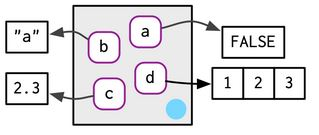
\includegraphics[height=.4\textheight]{envir.JPG}
\end{center}
A bit simplified: If a function is called, its own environment is created with its parent being the environment from which it was called.
\end{frame}


\begin{frame}[fragile]{Environments}
\begin{kframe}
\begin{alltt}
\hlstd{simple_fun} \hlkwb{<-} \hlkwa{function}\hlstd{()\{}
  \hlstd{a} \hlkwb{<-} \hlnum{1}
  \hlstd{b} \hlkwb{<-} \hlstr{"a"}
  \hlkwd{environment}\hlstd{()}
\hlstd{\}}
\hlstd{a} \hlkwb{<-} \hlkwd{simple_fun}\hlstd{()}
\hlstd{rlang}\hlopt{::}\hlkwd{env_print}\hlstd{(a)}
\end{alltt}
\end{kframe}<environment: 0000000014E820D8>
parent: <environment: global>
bindings:
 * b: <chr>
 * a: <dbl>

\end{frame}

\begin{frame}{Scoping}
Where does R find things?
\begin{itemize}
  \item Argument matching (name, place...)
  \item Current environment
  \item Parent environment
\end{itemize}
Programming advice:
Keep it simple, this can create chaos.
\end{frame}

\begin{frame}[fragile]{Scoping}
\begin{kframe}
\begin{alltt}
\hlstd{add_things2} \hlkwb{<-} \hlkwa{function}\hlstd{(}\hlkwc{x}\hlstd{) \{}
  \hlstd{x} \hlopt{+} \hlnum{10} \hlopt{+} \hlstd{y}
\hlstd{\}}
\hlkwd{add_things2}\hlstd{(}\hlnum{2}\hlstd{)}
\end{alltt}


{\ttfamily\noindent\bfseries\color{errorcolor}{\#\# Error in add\_things2(2): object 'y' not found}}\begin{alltt}
\hlstd{y} \hlkwb{<-} \hlnum{100}
\hlkwd{add_things2}\hlstd{(}\hlnum{2}\hlstd{)}
\end{alltt}
\end{kframe}[1] 112

\end{frame}

\begin{frame}{If clauses}
Conditional evaluation of code
\begin{itemize}
  \item Almost never useful outside of functions
  \item if() ... else ... can almost always be substituted by if() return
  \item Requires a logical of length 1
\end{itemize}
\end{frame}

\begin{frame}{If clauses}
Use cases
\begin{itemize}
  \item Input validation
  \item Different function behavior dependent on option arguments
  \item Requires a logical of length 1
\end{itemize}
\end{frame}

\begin{frame}[fragile]{If clauses}
\begin{kframe}
\begin{alltt}
\hlstd{mean2} \hlkwb{<-} \hlkwa{function}\hlstd{(}\hlkwc{x}\hlstd{,} \hlkwc{na.rm} \hlstd{=} \hlnum{FALSE}\hlstd{) \{}
  \hlkwa{if} \hlstd{(na.rm)\{}
    \hlstd{x} \hlkwb{<-} \hlstd{x[}\hlopt{!}\hlkwd{is.na}\hlstd{(x)]}
  \hlstd{\}}
  \hlkwd{sum}\hlstd{(x)}\hlopt{/}\hlkwd{length}\hlstd{(x)}
\hlstd{\}}
\end{alltt}
\end{kframe}
\end{frame}


\begin{frame}{Writing Functions}
  Before creating the function
  \begin{itemize}
    \item What should my function do?
    \item Input (Arguments)
    \item Output
  \end{itemize}
  After creating the function
  \begin{itemize}
    \item Test it
    \item Add input validation
    \item Document it
  \end{itemize}
\end{frame}

\section{Functions II}

\begin{frame}{What is a good function?}
\begin{itemize}
  \item pure functions
  \begin{itemize}
    \item no sideeffects
    \item no dependency on global environment
    \item easier understanding, easier transfer!
  \end{itemize}
\end{itemize}
\end{frame}

\begin{frame}{Debugging}
\begin{itemize}
  \item browser()
  \item traceback()
  \item options(error = recover)
\end{itemize}
\end{frame}

\section{Object Oriented Programming (S3)}

\section{Version Controlling (Git + Github)}
\begin{frame}{Motivation}
\begin{center}
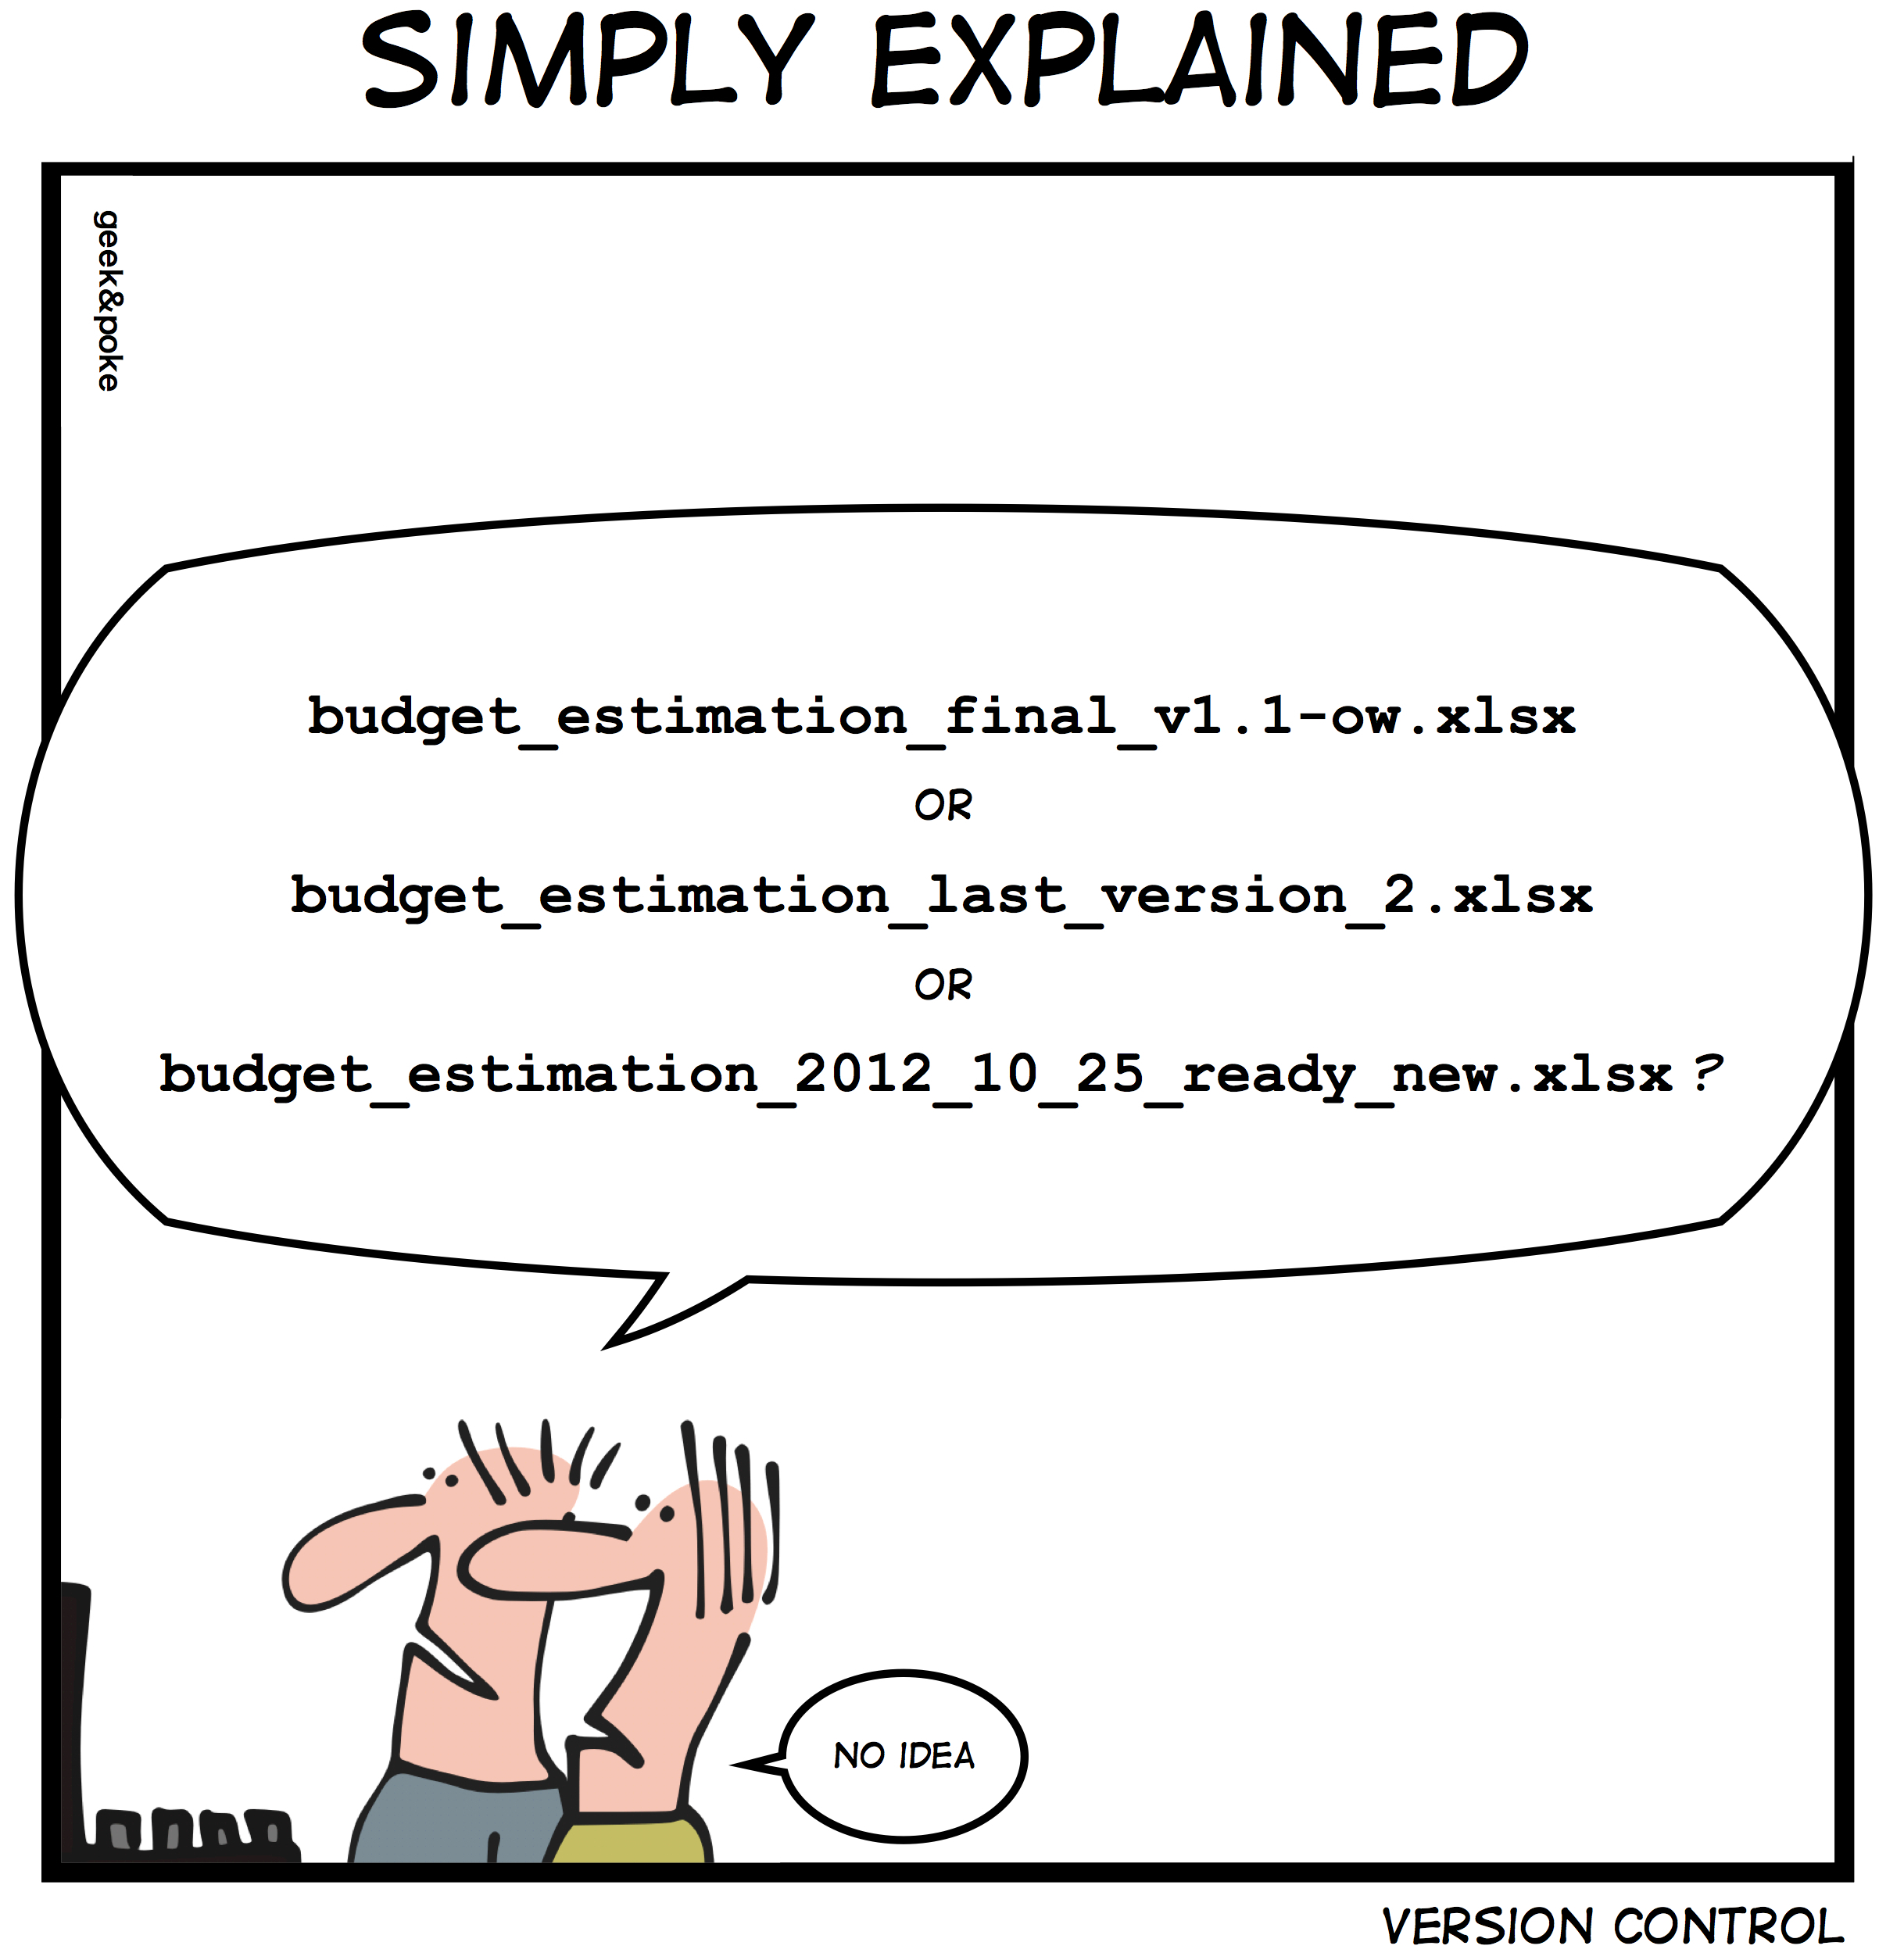
\includegraphics[height=.75\textheight]{why_version_control.jpg}
\end{center}
\end{frame}

\begin{frame}{Motivation}
\begin{itemize}
  \item Implementation of long term change history 
  \begin{itemize}
  \item No ridiculous file names
  \item No archive subfolder
  \item Always perfect overview of file history and changes
  \end{itemize}
  \item Collaborations
  \begin{itemize}
  \item What has changed?
  \item Who has changed it?
  \item Documentation of changes
  \item Parallel working possible (merging)
  \end{itemize}
\end{itemize}
\end{frame}

\begin{frame}{But...}
\begin{center}

\includegraphics[height=.75\textheight]{git_no_idea.png}
\end{center}
\end{frame}

\begin{frame}{Requirements}
\begin{itemize}
  \item Install git 
  \item Install User Interface for git (RStudio, Gitkraken, ...)
  \item Setup account for Github/Bitbucket/Gitlab/...
  \item Connect everything
\end{itemize}
\end{frame}

\begin{frame}{Workflow}
\textbf{Creating a repository}
\begin{itemize}
  \item Create an online repository (e.g. on Github)
  \begin{itemize}
    \item Use an R specific .gitignore
    \item Initialize with a short readme
  \end{itemize}
  \item Clone the repository to your local machine
  \item (optional) Place an R project in the existing repository
\end{itemize}
\end{frame}

\begin{frame}{Workflow}
\textbf{Working with a repository}
\begin{itemize}
  \item Before working: Synch your local repo (\textbf{Pull})
  \item Perform changes in your local repository
  \item \textbf{Stage} your changes
  \item \textbf{Commit} your changes (aka new version)
  \item \textbf{Push} your changes
\end{itemize}
\end{frame}

\begin{frame}{Recommendations}
\begin{itemize}
  \item Keep it simple! 
  \begin{itemize}
    \item No branches/forks/pull requests
  \end{itemize}
  \item Have meaningful commits
  \item Keep it lean (no big files)
\end{itemize}
\end{frame}

\begin{frame}{Resources}
Git (+ R) Resources
\begin{itemize}
\item Small Intro (\url{https://r-bio.github.io/intro-git-rstudio/})
\item Happy Git with R (\url{https://happygitwithr.com/})
\item R Packages and Git (\url{https://r-pkgs.org/git.html})
\item Git Book (\url{http://git-scm.com/book/en/v2})
\end{itemize}

\end{frame}

\begin{frame}{Literature Recommendations}
R Resources
\begin{itemize}
\item Avanced R Ed. 1 (\url{http://adv-r.had.co.nz/})
\item Avanced R Ed. 2 (\url{https://adv-r.hadley.nz/})
\item R Inferno (\url{https://www.burns-stat.com/pages/Tutor/R_inferno.pdf})
\item R Packages (\url{https://r-pkgs.org/})
\item Clean Code (\url{https://enos.itcollege.ee/~jpoial/oop/naited/Clean\%20Code.pdf)})
\end{itemize}

\end{frame}


\begin{frame}[plain]

\begin{center}
\Large Thank you for your attention!

\visible<2>{Questions? Remarks?}
\end{center}

\end{frame}

\end{document}
